\documentclass[a4paper,12pt]{article} 



\usepackage[utf8]{inputenc}
\usepackage[english, russian]{babel}
\usepackage{caption}
\usepackage{listings}
\usepackage{amsmath,amsfonts,amssymb,amsthm,mathtools }
\usepackage{wasysym}
\usepackage{graphicx}
\usepackage{float} 
\usepackage{wrapfig} 
\usepackage{fancyhdr} 
\usepackage{lscape}
\usepackage{xcolor}
\usepackage[normalem]{ ulem }
\usepackage{hyperref}





\hypersetup
{
    colorlinks = true,
    linkcolor = blue,
    filecolor = magenta,
    urlcolor = blue
}


\pagestyle{fancy}
\fancyhead{}
\fancyhead[L]{ 2.2.8 }
\fancyhead[R]{ Талашкевич Даниил, 2 положительная группа крови}
\fancyfoot[C]{ \thepage }



\begin{document}


\begin{titlepage}

\newpage
\begin{center}
\normalsize Московский физико - технический институт //госудраственный университет)
\end{center}

\vspace{6em}

\begin{center}
\Large Домашняя работа по Физической культуре\\
\end{center}

\vspace{1em}

\begin{center}
\large \textbf{ Исследование термических эффектов,
возникающих при упругих деформациях[2.2.8] }
\end{center}

\vspace{2em}

\begin{center}
\large П$ ^ 3$ : Полная Полтрашка Патриковна и Талашкевич Даниил Александрович \\
Группа Б01 - \href{ https://vk.com/rt_kiska }{\textbf{Гладим киску каждый день}}
\end{center}

\vspace{\fill}

\begin{center}
    \large Иерусалим \\ 2 век до н.э.
\end{center}

\end{titlepage}



    \thispagestyle{empty}
    \newpage
    \tableofcontents
    \newpage
    \setcounter{page}{1}


\section{Введение в историю Иерусалима}

Древнейшая часть Иерусалима была заселена в 4-м тысячелетии до н.э., что делает его одним из древнейших городов мира. За свою долгую историю, Иерусалим был как минимум дважды разрушен, 23 раза осаждён, 52 раза атакован и 44 раза завоёван либо вновь отвоёван.

В разное время городом владели Израильское царство, Иудейское царство, Вавилон, Персидская империя и империя Александра Македонского, Египет Птолемеев, Сирия Селевкидов. После еврейского восстания во II веке до н.э. на некоторое время было восстановлено Иудейское Царство, но уже в 6 году н.э. на месте него была провозглашена римская провинция Иудея. Вслед за распадом Римской империи, Иерусалим отошёл к Византии. После Византии город принадлежал арабским халифатам, крестоносцам, государствам Айюбидов и мамлюков, Османской и затем Британской империям, Иордании и, наконец, Израилю.

 Учитывая центральное место, отводимое Иерусалиму как еврейским, так и палестинским национализмом, на избирательность, неизбежную при резюмировании более чем 5000 - летней истории его населённости, часто накладывается идеологическая предвзятость или предшествующий опыт авторов.Еврейские периоды истории города важны для израильских националистов, дискурс которых предполагает, что современные евреи происходят от израэлитов и Маккавеев в то время как исламский, христианский и другие нееврейские периоды его истории важны для палестинского национализма, дискурс которого производит современных палестинцев от всех разнообразных народов, населявших регион. В результате каждая из сторон утверждает, что история города была политизирована оппонентами, дабы подкрепить притязания последних на город, и что это подтверждается разностью акцентов, придаваемых различными авторами разнообразным событиям и эрам в истории города.

\section{Как древние греки считали производные}
Для того, чтобы вычислять производную греки поступили очень умно : они построили машину времени, переместились в 2021 год н.э., затем на крысичях украли мой \textbf{exe}-шник и данную статью с подробнейшим описанием как искать ее в 2021 году, затем вернулись обратно и сковозь долгие годы они научились все - таки ее брать.Вы наверное подумаете, что это все чисто воды обман и выдумка, но у меня есть на то доказательства : \newpage

 \begin{figure}[h]
 \center{ 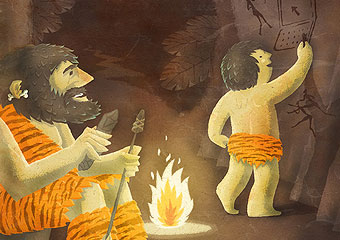
\includegraphics[scale = 1]{proof.jpg} }
 \label{ photo1:1 }
 \end{figure}

 На данном фото видно, как они внаглую просто переписывают мой код!!!! P.S.Фото взято из архивов национального музея наследний ЮНЕСКО

\section{Как вычислить производную в 2021 году}

Сейчас научим тупых греков считать прозводную на следующем примере:
\begin{equation}
\left(2+1\right)^{\ln(x-1)  \cdot x} 
\end{equation} 

Чтобы получить ответ необходимо сделать сложный мув, а именно взять эту производную:
\begin{equation}
\left(2+1\right)^{\ln(x-1)  \cdot x} 
\end{equation} 
Степень-степень-степень, что же делать с этим? Для этого заглянем в АнтиДемидовича, том 1, страница 112, примеры 1-2

Но чтобы не париться с различными случаями можно ее взять в обшем случае:

  \begin{equation}
  f(x)^{g(x)} = e^{g(x)\cdot ln(f(x))}  = f(x)^{g(x)} \cdot \left(g(x)\cdot ln(f(x)) \right)^{'} =  
 \end{equation} \\Значит нужно рассчитать следующую производную:

\begin{equation}
\ln(x-1)  \cdot x \cdot \ln(2+1) 
\end{equation} 
Чтобы попа не потела, не кусали комары, полторашка научит вас брать диффуры. Шучу! Мы возьмем следующую производную:
\begin{equation}
\ln(x-1)  \cdot x \cdot \ln(2+1) 
\end{equation} 
На научной конференции 982 года по квантовой термодинамике Пушкин доказал, что мы живем в 3.14-мерном пространстве и оно кошка-симметрично, отсюда как раз-таки следует, что производная от произведения это:

  \begin{equation}
  f(x) \cdot g(x) = f^{'}(x) \cdot g(x) + f(x) \cdot g^{'}(x)
 \end{equation} \\Поэтому по методу Центрирования галактик рассчитаем производную f(x), которое равна: 
\begin{equation}
\ln(x-1)  \cdot x
\end{equation} 
Чтобы попа не потела, не кусали комары, полторашка научит вас брать диффуры. Шучу! Мы возьмем следующую производную:
\begin{equation}
\ln(x-1)  \cdot x
\end{equation} 
На научной конференции 982 года по квантовой термодинамике Пушкин доказал, что мы живем в 3.14-мерном пространстве и оно кошка-симметрично, отсюда как раз-таки следует, что производная от произведения это:

  \begin{equation}
  f(x) \cdot g(x) = f^{'}(x) \cdot g(x) + f(x) \cdot g^{'}(x)
 \end{equation} \\Поэтому по методу Центрирования галактик рассчитаем производную f(x), которое равна: 
\begin{equation}
\ln(x-1) 
\end{equation} 
Опираясь на Кудрявцева, том 1, страница 112, пример 11 можно получить производную логарифма.

Как в детстве нас учили ходить, так и сейчас мы возьмем следующую производную:
\begin{equation}
x-1
\end{equation} 
Даже Рома Глаз знает, что производная от суммы или разности равна соответственно сумме/разности производных ее частей\\Поэтому посчитаем производную слева: 
\begin{equation}
x
\end{equation} 
В свою же очередь производная от переменной = $- \cos(\pi) + \sin(0) = 1$.

Её производная с точностью до распределение Ферми-Дирака получается равной:
\begin{equation}
1
\end{equation} 
А после, если останутся силы, производную правой части, которая равна: 
\begin{equation}
1
\end{equation} 
Ссылаясь на 2 том Кудрявцева, производная от константы = $e^{i\pi} + 1 = 0$.

На лекции по русской литературу я узнал об законе больших чисел Бернулли-Горяйнова, из которого следует следующее выражение для производной:
\begin{equation}
0
\end{equation} 
 P.S. тут полторашка словила шизу и начала бегать по комнате, поэтому за правильность результата она не ручается. С погрешностью в 0.1 почку вискаса получаем:
\begin{equation}
\frac{1-0}{x-1} 
\end{equation} 
Ну так как Mrs.Patrikovna сейчас бегает за своим хвостом, то следующую производную: 
\begin{equation}
x
\end{equation} 
В свою же очередь производная от переменной = $- \cos(\pi) + \sin(0) = 1$.

Остальную часть я попробую взять сам, в этом мне поможет баночка охоты крепкого. *Буль-Буль*, получаем что-то такое:
\begin{equation}
1
\end{equation} 
 P.S. тут полторашка словила шизу и начала бегать по комнате, поэтому за правильность результата она не ручается. С погрешностью в 0.1 почку вискаса получаем:
\begin{equation}
\frac{1-0}{x-1}  \cdot x+1 \cdot \ln(x-1) 
\end{equation} 
Ну так как Mrs.Patrikovna сейчас бегает за своим хвостом, то следующую производную: 
\begin{equation}
\ln(2+1) 
\end{equation} 
Опираясь на Кудрявцева, том 1, страница 112, пример 11 можно получить производную логарифма.

Как в детстве нас учили ходить, так и сейчас мы возьмем следующую производную:
\begin{equation}
2+1
\end{equation} 
Даже Рома Глаз знает, что производная от суммы или разности равна соответственно сумме/разности производных ее частей\\Поэтому посчитаем производную слева: 
\begin{equation}
2
\end{equation} 
Ссылаясь на 2 том Кудрявцева, производная от константы = $e^{i\pi} + 1 = 0$.

Её производная с точностью до распределение Ферми-Дирака получается равной:
\begin{equation}
0
\end{equation} 
А после, если останутся силы, производную правой части, которая равна: 
\begin{equation}
1
\end{equation} 
Ссылаясь на 2 том Кудрявцева, производная от константы = $e^{i\pi} + 1 = 0$.

На лекции по русской литературу я узнал об законе больших чисел Бернулли-Горяйнова, из которого следует следующее выражение для производной:
\begin{equation}
0
\end{equation} 
Остальную часть я попробую взять сам, в этом мне поможет баночка охоты крепкого. *Буль-Буль*, получаем что-то такое:
\begin{equation}
\frac{0+0}{2+1} 
\end{equation} 
В итоге получаем следующим результат:
\begin{equation}
\left(\frac{1-0}{x-1}  \cdot x+1 \cdot \ln(x-1) \right) \cdot \ln(2+1) +\frac{0+0}{2+1}  \cdot \ln(x-1)  \cdot x
\end{equation} 
После двух бессонных ночей, шести пачек вискаса и бутылки охоты крепкого Мы получили примерно следующее:
\begin{equation}
\left(\left(\frac{1-0}{x-1}  \cdot x+1 \cdot \ln(x-1) \right) \cdot \ln(2+1) +\frac{0+0}{2+1}  \cdot \ln(x-1)  \cdot x\right) \cdot \left(2+1\right)^{\ln(x-1)  \cdot x} 
\end{equation} 
Но данное выражение какое-то некрасивое, поэтому давайте его преобразуем к следующему виду:
\begin{equation}
\left(\frac{1}{x-1}  \cdot x+\ln(x-1) \right) \cdot \ln3 \cdot 3^{\ln(x-1)  \cdot x} 
\end{equation} 
\section{Заключение}
 При выполнение домашней работы по физической культуре я узнал про историю Иерусалима, познакомился с тем, как греки считали производные, а так же сам научился считать производную по шагам!
\section{Используемые тренажеры}
 \begin{enumerate}
 \item Скакалка
 \item Эскандер
 \item Крижометр (отдельное спасибо Крижовичу за то, что предоставил его мне!)
 \item Коксовая дорожка
 \end{enumerate}
\end{document}
